\documentclass[a4paper, 12pt]{article}
\usepackage[utf8]{inputenc}
\usepackage{multicol}
\usepackage{pgf}
\usepackage{pgfpages}
\usepackage{wrapfig}
\usepackage{tikz}
\usetikzlibrary{calc,arrows}
\usepackage{multicol}
\usepackage{lipsum} 
\usepackage{graphicx}
\usepackage[margin=20mm]{geometry}
\usepackage{subfig}
\usepackage{xcolor}
\usepackage{ntheorem} 
\usepackage{mdframed} 
\usepackage{blindtext}
\usepackage{exercise}

\begin{document}
\centering
\colorbox{white!10!}{
    \begin{minipage}[H]{\textwidth}
        \begin{center}
            {\large \textsc{University of Moratuwa}}\\
            {\large \textsc{EN2550 - Fundamentals of Image Processing and Machine Vision}}
            \vspace{0.25cm}
            \\
            { \huge \textbf{Assignment II}}
            \\
            \vspace{0.25cm}
            \small Name - Weerasinghe K.N.\\
            \small Index No. - 190672T
        \end{center}
    \end{minipage}
}
\begin{center}
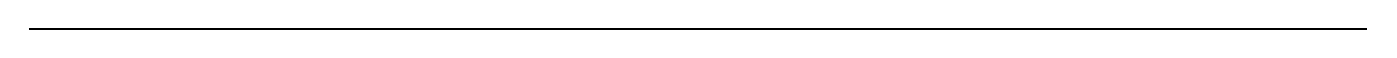
\begin{tikzpicture}
    \draw[thick] (-10.5,0)--(6.5,0);
\end{tikzpicture}
\end{center}

\begin{wrapfigure}{r}{5 cm}
    \centering
    \includegraphics[width=4 cm]{Images/Q1 - RANSAC.png}
    \caption{\centering PIR sensor module}
    \label{fig:im1}
\end{wrapfigure}

\begin{description}
   \item[Question 1 :] The code snippet in Listing 1 shows the code to generate a noisy point set X amounting to a circle and the code to estimate a circle—center and the radius—from a set of inliers in X.\\
(a) Estimate the circle using the RNASAC algorithm (must be coded on your own).\\
(b) Show in the same plot, the point set, the circle estimated from the sample leading to the best estimate, this sample of three points, inliers, and the best-fit circle. See Figure 1 for an example.
    
\item[Answer :] \blindtext
    
%----------------------------------------------------------------

    \item[Question 2 :]  Figure 2 shows an architectural image1 with a flag 2
superimposed. This is done by clicking four points on a planar surface in the architectural image, computing a homography that maps the flag image to this plane,
and warping the flag, and blending on to the architectural image. Carry this out for a couple of image pairs of you own choice. You may explain the (non-technical) rationale of your choice
    \item[Answer :]
    
%----------------------------------------------------------------

    \item[Question 3 :] In this questions, we will stitch the two Graffiti image3
img1.ppm onto img5.ppm.\\
(a) Compute and match SIFT features between the two images.\\
(b) Compute the homography using your own code within RANSAC and compare with the homography given in the dataset.\\
(c) Stitch img1.ppm onto img5.ppm
    \item[Answer :]
\end{description}

\end{document}